\section{Resultados} \label{resultados}

A mesma base de teste (sendo 10 de cada classe, totalizando 30) foi usada para verificar tanto o desempenho das 3 redes que compõe a auto associativa quanto da rede MLP.

O parâmetro de comparação foi o erro médio quadrático (MSE) obtido no desempenho das redes.


\subsection{Desempenho da Rede MLP}

A rede MLP apresentou um desempenho bom, tendo em vista que houve apenas 1 erro na classificação.

\begin{figure}[H]

\centering % para centralizarmos a figura
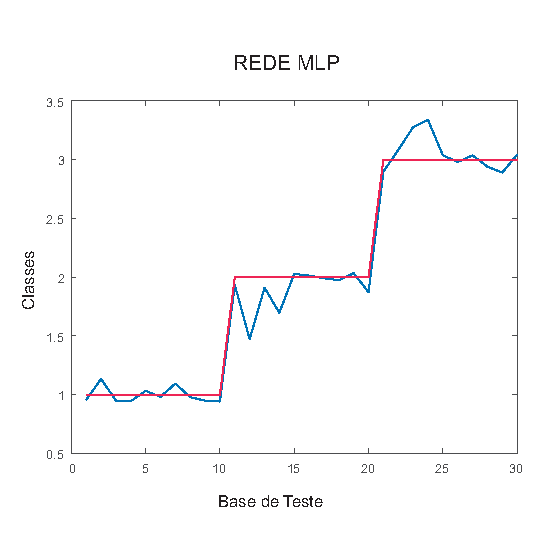
\includegraphics{04-Figuras/SAIDA_MLP}

\caption{Saída da rede MLP}

\label{figura:saidaMLP}

\end{figure}

A fig. \ref{figura:saidaMLP} mostra o desempenho da rede MLP, onde em azul é a saída da rede e em vermelho, a saída desejada.


\subsection{Desempenho da Rede Auto Associativa}

Considerando toda a base de teste (30 instâncias), as três redes que compõe a estrutura competitiva auto associativa apresentaram resultados bem interessantes para as classes nas quais elas são especializadas. No entanto, elas apresentaram erros consideráveis para as instâncias da base de teste pertencente às outras classes (o que de certa forma é esperado).


\subsubsection{Desempenho da Rede 1}

A fig. \ref{figura:rede1} mostra o desempenho da rede 1, que é especializada na classe 1.

\begin{figure}[H]

\centering % para centralizarmos a figura
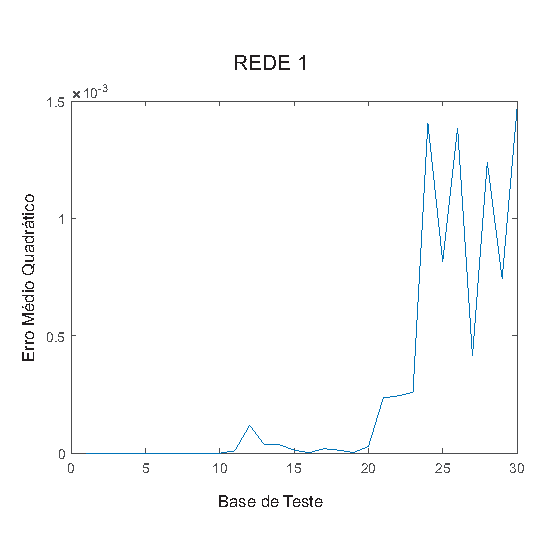
\includegraphics{04-Figuras/MSE_DesempenhoNet1}

\caption{Desempenho da rede 1}

\label{figura:rede1}

\end{figure}

Observa-se que o erro médio quadrático é extremamente baixo para a base de dados de 1 a 10 (que corresponde à classe 1) e bastante significativo entre 11 a 30, que são instâncias pertencentes às classes 2 e 3.

\subsubsection{Desempenho da Rede 2}

Na rede 2, o padrão de comportamento da rede 1 se repetiu. Observa-se que de 1 a 10 o MSE é acentuado, sendo extremamente baixo de 11 a 20 (instâncias pertencentes à classe 2), e novamente alto de 21 a 30, como mostrado na fig. \ref{figura:rede2}.

\begin{figure}[H]

\centering % para centralizarmos a figura
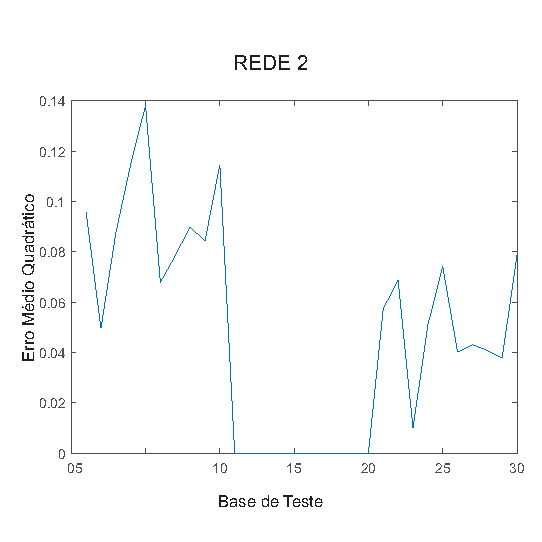
\includegraphics{04-Figuras/MSE_DesempenhoNet2}

\caption{Desempenho da rede 2}

\label{figura:rede2}

\end{figure}

\subsubsection{Desempenho da Rede 3}

Seguindo a tendência de comportamento, a rede 3 apresentou um alto valor do MSE para as instâncias de 1 a 20 (pertencentes às classes 1 e 2), bem como um erro muito baixo para as instâncias da classe 3, onde a rede 3 é especializada, de 21 a 30.

\begin{figure}[H]

\centering % para centralizarmos a figura
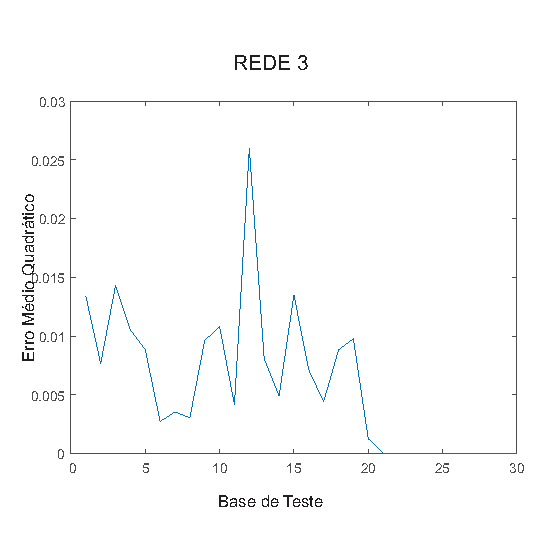
\includegraphics{04-Figuras/MSE_DesempenhoNet3}

\caption{Desempenho da rede 3}

\label{figura:rede3}

\end{figure}



\subsection{Comparação Rede MLP X Rede Auto Associativa}

Varius erat fames feugiat pellentesque eros laoreet lacinia integer condimentum sed vulputate, integer condimentum eleifend maecenas dapibus viverra nunc rhoncus eros. volutpat consectetur dictum purus etiam augue ipsum litora consectetur commodo mi, commodo est cursus sem ac cubilia conubia in at. ligula fermentum nisl erat sed posuere ac fusce sociosqu, porttitor vulputate tellus platea duis tristique tellus. vehicula varius pellentesque nam sapien aptent, et vivamus eget turpis ac, sit bibendum eros varius. venenatis ultrices dui sollicitudin aliquam pellentesque sagittis elit sociosqu ut, lorem consectetur adipiscing eu elementum ipsum nullam eros, egestas ligula dapibus congue est ornare vitae hendrerit.

Tabela de comparação